\documentclass[final]{ubb_dolgozat}
\usepackage{definitions}
\usepackage{url}
\sloppy
\frenchspacing

\lstloadlanguages{Java}

\lstset{language=Java}

\submityear{
2016
}
\submitmonthHU{
Július
}
\submitmonthRO{
Iulie
}
\submitmonthEN{
July
}

\titleHU{
Kontroll és egyensúlyozás -- alkalmazás Lego robotnál
}

\titleEN{
Control and balancing -- applied to Lego robots
}

\titleRO{
Control \c{s}i echilibrare -- aplicat la robo\c{t}i Lego
}

\author{
Márton Zete-Örs
}

\tutorHU{
dr. Jakab Hunor,\newline egyetemi adjunktus\\
}
\tutorRO{
Lector dr. Hunor Jakab\\
}
\tutorEN{
Assist prof. dr. Hunor Jakab
}

\begin{document}

\begin{abstractEN}
	
A szakdolgozat célja egy egyensúlyozó, kétkerekű MINDSTORMS EV3 robot irányításának megoldása hálózaton keresztül, telefonos alkalmazás segítségével. Ennek a célnak az eléréséhez szükséges két nagyobb feladat elvégzése. A kommunikációt megvalósító telefonos alkalmazás elkészítése illetve az egyensúlyba tartó algoritmus implementálása.

Az alkalmazás és az egyensúlyozást megvalósító algoritmus Java-ban íródott. A robot irányításáért felelős az EV3 vezérlőegység, amelyen Linux alapú leJOS keretrendszer fut. A robot PID (\texttt{Proportional Integral Derivative}) kontroller alkalmazásával és giroszkóp szenzor használatával marad egyensúlyban. Ahhoz hogy egyensúlyba maradjon a robot sebessége, dőlési szöge, szög változásának a sebessége 0-hoz kell közelítsen illetve annak az érdekében, hogy egy helyebe maradjon pozíciója is 0-hoz kell tartson.
A PID bemeneti értéke a hiba, amely az elvárt érték és az aktuális érték különbsége. Esetünkben mivel 0-t kell közelítsünk annak érdekében, hogy ne veszítse el egyensúlyi állapotát a robot ezért az elvárt érték öröké 0 lesz, vagyis a hibát négy komponens alkotja: a robot dőlési szöge, szögsebessége, a robot sebessége és pozíciója. A komponensek megfelelő módosítása lehetővé teszi a robot mozgásának manipulálását. 

Mobil részre egy telefonos alkalmazást fejlesztettünk, amely hálózaton keresztül kapcsolódik a robothoz és küldi a megfelelő parancsokat. Az alkalmazás és a robot közti kapcsolat létrehozásának automatizálására UPnP(\texttt{Universal Plug and Play}) könyvtárat használjuk, amely SSDP(\texttt{Simple Service Discovery Protocol}) protokollt használ.

This work is the result of my own activity. I have neither given nor received unauthorized assistance on this work.

\end{abstractEN}

\maketitle

{ \baselineskip 1ex
  \parskip 1ex
  \tableofcontents
}

\chapter{Bevezető}
A szakdolgozat által bemutatásra kerül egy projekt, amely a LEGO MINDSTORMS EV3\cite{mindstormsEv3} készletből épített kétkerekű egyensúlyozó robot irányítását teszi lehetővé hálózaton keresztül, telefonos alkalmazás segítségével. Emellet sor kerül a robot főbb elemeinek a bemutatása, felhasznált technológiák és a vezérlést kezelő Android alkalmazás.

A kétkerekű robot a Gyro Boy\footnote{\href{http://robotsquare.com/wp-content/uploads/2013/10/45544\_gyroboy.pdf}{http://robotsquare.com/wp-content/uploads/2013/10/45544\_gyroboy.pdf}} modell alapján készült el. Főbb komponensei közé sorolható az EV3 vezérlőegység\footnote{\href{http://lego.wikia.com/wiki/45500\_EV3\_Intelligent\_Brick}{http://lego.wikia.com/wiki/45500\_EV3\_Intelligent\_Brick}}, giroszkóp szenzor\footnote{\href{http://shop.lego.com/en-US/EV3-Gyro-Sensor-45505}{http://shop.lego.com/en-US/EV3-Gyro-Sensor-45505}} és a két nagy szervomotor\footnote{\href{http://lego.wikia.com/wiki/45502\_EV3\_Large\_Servo\_Motor}{http://lego.wikia.com/wiki/45502\_EV3\_Large\_Servo\_Motor}}, amelyek párhuzamosan vannak elhelyezve. Az előbb említett elemekről bővebben szó lesz a \ref{sec:ROBOT:motorok} illetve \ref{sec:ROBOT:szenzorok} fejezetben. Mivel a kerekek párhuzamosan helyezkednek el ezért nem marad egyensúlyi állapotban. E probléma megoldására alkalmas a PID\footnote{\href{https://en.wikipedia.org/wiki/PID\_controller}{https://en.wikipedia.org/wiki/PID\_controller}} szabályzó algoritmus használata, amely ipari körökben elterjedt a viszonylag egyszerű felépítéséért, kezelhetőségéért és implementálhatóságáért. A szabályzó bemeneti értékét az aktuális hiba határozza meg, amelyet négy értékből határozunk meg: szög, szögsebesség, robot sebesség és a robot pozíciója, amelyek külön-külön súlyozva vannak. A szög és szögsebesség érték meghatározásához szükséges a giroszkóp szenzor és a szervomotorok beépített szenzorjai teszik lehetővé a sebesség és pozíció megállapítását.

A robot irányításának érdekében szükséges a PID szabályzó algoritmus módosítása és esetleges újabb szabályzók bevezetése annak érdekében, hogy irányítás alatt ne veszítse el az egyensúlyi állapotát. A felhasználónak lehetőséget ad a projekt Android alkalmazása, hogy hálózaton, socketeken keresztül csatlakozzon a robothoz és az irányításnak megfelelő adatokat továbbítsa. Ezen adatok beviteli módját egy "touch joystick" teszi lehetővé, amellyel négy irányba lehetséges a robot vezérlése. Az adatok védelmét, a tovább bővíthetőséget illetve a szerializációt a Google Protocol Buffers\footnote{\href {https://developers.google.com/protocol-buffers/}{https://developers.google.com/protocol-buffers/}} biztosítja. A Protocol Buffers platform és nyelvfüggetlen, könnyen kezelhető és gyors. Lehetőséget nyújt az adatok tetszőleges felépítésére, amelynek a forráskódját egy speciális generátor segítségével könnyen kigenerálható. E strukturált adatok írását illetve olvasását biztosítja a generált kód.

Az EV3 készlethez biztosított a LEGO MINDSTORMS egy grafikus felületet, amellyel a kisebb korosztály "programozhatja" a saját kezűleg épített robotokat. E projekt esetében leJOS \footnote{\href {https://en.wikipedia.org/wiki/LeJOS}{https://en.wikipedia.org/wiki/LeJOS}} keretrendszer fut az EV3 vezérlőegységen. A leJOS Linux alapú és magába foglalja a JVM-t (Java virtual machine), amely lehetővé teszi, hogy a robot programozható legyen Java-ban. 

A dolgozat 3 fejezetből áll. Az első fejezet bevezetőként szolgál a projektbe.

A második fejezet röviden bemutatja a LEGO megalakulását, a LEGO MINDSTORMS által kifejlesztett generációkat majd bemutatja az EV3 készlethez tartozó motorokat és szenzorokat. Tartalmazza azon eszközök részletes leírását amelyek a projekt által használatosak.

A harmadik fejezet által bemutatásra kerül a PID szabályzó működése és használata e projekt esetén.
\chapter{LEGO} \label{ch:ROBOT}

\begin{osszefoglal}
A fejezetben bemutatásra kerül a LEGO megalakulása, fejlődése. E mellett sor kerül a LEGO MINDSTORMS által kifejlesztett technológiák bemutatására, amelyek közül a giroszkóp szenzor és a nagy motorok felhasználásra kerülnek a továbbiakban.
\end{osszefoglal}

\section{LEGO megalakulása}\label{sec:ROBOT:lego}
A LEGO~\cite{lego}\cite{legoHistory} története 1932-ben kezdődött, Ole Kirk Christiansen\footnote{\href {http://lego.wikia.com/wiki/Ole\_Kirk\_Christiansen}{http://lego.wikia.com/wiki/Ole\_Kirk\_Christiansen}} asztalos vállalkozást alapított Dánia, Billund nevezetű falujában, amely a fa játékok gyártásával foglalkozott. 1934-ben vette fel a cég a LEGO nevet, amely a LEG GODT dán szóból ered. 1947 után kezdtek el műanyagból előállítani játékokat, amelyek fő célja az volt, hogy könnyedén egymásba illeszthetőek, illetve szétszedhetőek legyenek. Az alapító fia, Godtfred Christian, lett az igazgató 1958-ban, ekkor alakult meg a ma ismert LEGO vállalat és vezetésével fellendült a cég. Az első számítógép által vezérelt robot 1986-ban jelent meg, amelyet követően 1988-ban a LEGO és az MIT \texttt{(Massachusetts Institute of Technology)} együttműködésével elkezdődött az "inteligens tégla" fejlesztése, mely lehetőséget ad a programozhatóságra.

\section{LEGO MINDSTORMS}\label{sec:ROBOT:mindstorms}
A LEGO  első játéka, amit forgalmazott Ole Kirk Christians vezetésével, a fából készült "LEGO Duck". Évekkel később megjelentek a műanyag játékok. Ma már világszerte ismert a LEGO építőjáték, egymással összeilleszthető, kombinálható elemeket tartalmaz, így szinte bármi megépíthető belőle és rendkívül hasznos oktatási eszköz. 

A LEGO MINDSTORMS~\cite{mindstormsHistory} egy programozható robotikai építőkészlet. Lehetőséget ad arra, hogy megépítsd, programozd és irányítsd a robotot.
1998-ban jelent meg az első generáció, az RXC \texttt{(Robotic Command eXplorers)}, akkoriban nagy előrelépést számított, mivel teljesen autonóm. Képes számítógép nélkül is működni de, mára már nem gyakori a használata. Az évek során sokat fejlődött és ma már egyre több oktatási intézmény használja a robotika oktatásban.

\subsection{RXC}
Az RXC~\cite{rxcAttribution}, amelyet a \ref{fig:RXC} ábra szemlélteti, az első generációs LEGO MINDSTORMS. Ma már nem igen használatos, elavult programozható vezérlőegység, mivel csupán 8 bites mikrokontroller és 32 Kbyte RAM-al rendelkezik. Tartalmaz három szenzor és három motor csatlakozó portot. Ezek mellett egy LCD kijelzőt, amin látható az akkumulátor töltöttségi szintje, a bemeneti és kimeneti portok állapota. Egyéb információk megjelenítésére is alkalmas. A kapacitásának ellenére számos projektben felhasználták, ilyenekben mint például a \texttt{Brick Sorter}\footnote{\href {http://robotsquare.com/2012/02/15/brick-sorter-4/}{http://robotsquare.com/2012/02/15/brick-sorter-4/}}, amely szín szerint szortírozza az adott elemeket, \texttt{RCX Remote Control}\footnote{\href {http://robotsquare.com/2012/02/14/rcx-remote-control/}{http://robotsquare.com/2012/02/14/rcx-remote-control/}}, amely két RCX vezérlőegység közti kommunikációval irányítja a robot.

\begin{figure}[!htb]
	\centering
	\pgfimage[width=0.4\linewidth]{images/RXC}
	\caption{RXC brick}
	\label{fig:RXC}
\end{figure}

\subsection{NXT}
A második generáció a \ref{fig:NXT} ábrán látható, az NXT~\cite{nxtAttribution}\cite{nxtVsEv3}, 2006-ban jelent meg illetve az NXT 2.0 2009-ben, amely több építőelemet és szenzort tartalmaz. Több mindenben különbözik az NXT az RXC-hez képest. Szembetűnő esztétikai változások történtek, javítottak a kapacitáson, növelték a portok számát és megjelentek a szervomotorok.

Az NXT tartalmaz négy bemeneti portot, három kimeneti portot és egy 2.0 USB portot. Beépített bluetooth kommunikációs adapterrel rendelkezik, megjelent a grafikus kijelző és tartalmazott egy 8Khz hangszórót. Az NXT 32 bites AMTEL ARM7 mikrokontrollerrel, 256 Kbyte flash memóriával és 64 Kbyte RAM-al rendelkezik. Az NXT csomaggal már komplexebb projektek is készültek, mint az RXC-vel. Megemlíteném a \texttt{Segway with Robot Driver}\footnote{\href {http://robotsquare.com/2012/09/04/segway-with-robot-driver/}{http://robotsquare.com/2012/09/04/segway-with-robot-driver/}} című projektet, amely megvalósított egy olyan robotot, amely irányítja a szintén NXT vezérlőegység által működtetett Segway-t.

\begin{figure}[!htb]
	\centering
	\pgfimage[width=0.4\linewidth]{images/NXT}
	\caption{NXT brick}
	\label{fig:NXT}
\end{figure}

\subsection{EV3}

A harmadik generáció, az EV3~\cite{ev3Attribution}\cite{nxtVsEv3} 2013-ban jelent meg, a \ref{fig:EV3} ábra szemlélteti. Az "EV" evolúciót jelent és a 3-as azt, hogy harmadik generáció. Az EV3 a legfejeltebb LEGO MINDSTROMS programozható építőelem, amely kezeli a motorokat, a szenzorokat és lehetőséget ad Bluetooth-on keresztül való kommunikációra.

Az EV3 egy ARM9 nevű processzorral van felszerelve, amely 300 Mhz, 16 Mbyte flash memóriával és 64 Mbyte RAM-al rendelkezik. A Linux alapú operációs rendszere nagyban segíti a programozhatóságát. Egy 2.0 mini USB PC porton teszi lehetővé a számítógéppel való kommunikációt, aminek átviteli sebessége 480 Mbit/s, az SD kártya olvasója 32 Gbyte-ot ismer fel. Tartalmaz egy USB portot amely lehetővé teszi, hogy használjunk Wi-Fi dongle-t, ezáltal megkönnyíti a programok kitelepítését, fájlok kezelését és lehetségessé teszi a kommunikációt okos készülékekkel is.

Az NXT-hez képest sokat fejlődött, nagyobb a kapacitása, lehetőség van Wi-Fi és SD kártya használatára. Ezek mellet négy szenzor port van három helyett és négy motor csatlakozó port. Nagyobb LCD kijelzőt raktak és a felületén hat gomb van négy helyett, könnyítve az operációs rendszer menüjének kezelését.\cite{nxtVsEv3}

Mivel a LEGO MINDSTORMS generációk közül a legfejlettebb ezért a projekt által felhasznált vezérlőegység az EV3.

\begin{figure}[!htb]
	\centering
	\pgfimage[width=0.4\linewidth]{images/EV3}
	\caption{EV3 brick}
	\label{fig:EV3}
\end{figure}


\section{Ev3 motorok}\label{sec:ROBOT:motorok}
Az NXT generációval megjelentek a szervomotorok, amelyek legfőbb tulajdonsága a pontosság. Két típusa jelent meg a közepes és a nagy szervomotor. Mind a kettőnél megmaradt a pontosság, de a méretük, az erejük és a reagálási idejük eltérnek. Tovább fejlesztették a motorokat, amelyek az EV3 generációval jelentek meg. Az EV3 nagy motorjának teljesítménye megegyezik az NXT-vel de a felépítését optimalizálták, illetve az EV3 közepes motorja teljesen új az NXT-hez képest.

\subsection{Nagy motor}
A nagy motor, amelyet a \ref{fig:lMotor} ábrázol, erőteljes, ideális az általunk megépített robot irányítására. A motorba beépített forgásérzékelő által  információkat lehet lekérni a pillanatnyi állapotáról, amely fokban vagy teljes fordulatban mér.

A nagy motorok sebessége 160-170 rmp, forgatónyomatéka 20 N/cm és, ha blokkolt állapotba kerül, akkor a nyomatéka 40N/cm. A motor beépített forgásérzékelője lehetővé teszi a pontos vezérlést +/- 1 fok pontossággal.

A robot mozgatását a nagy motorok segítségével fogjuk elérni, habár lassabbak, mint a közepes motorok, de nagyobb a nyomatékuk és a precizitásuk azonos.

\begin{figure}[!htb]
	\centering
	\minipage{0.4\textwidth}
	\pgfimage[width=0.9\linewidth]{images/large_motor}
	\caption{Nagy motor}
	\label{fig:lMotor}
	\endminipage
	\minipage{0.4\textwidth}
	\pgfimage[width=0.8\linewidth]{images/medium_motor}
	\caption{Közepes motor}
	\label{fig:mMotor}
	\endminipage
\end{figure}

\subsection{Közepes motor}
A közepes motor, amelyet a \ref{fig:mMotor} ábrázol, tulajdonsági megegyeznek a nagy motor tulajdonságaival. Ugyancsak tartalmaz forgásérzékelőt és lehetséges a helyzetmeghatározás 1 fok eltéréssel, viszont alacsonyabb terhelésre tervezték, forgatónyomatéka 8 N/cm, ha blokkolt állapotba kerül, akkor a nyomatéka 12 N/cm és a sebessége 240-250 rmp.

\section{Ev3 szenzorok}\label{sec:ROBOT:szenzorok}

Az NXT csomagban számos szenzor megtalálható, ilyenek az érintés, a hang, a szín és az ultrahang szenzorok, amelyeket felhasználva több különböző funkcionalitásokkal bővíthetjük a megépített robotunkat. Az EV3 megjelenése magával hozott még két új szenzort, a giroszkóp és az infravörös szenzorokat. Ezek mellett fejlesztették a már meglévő szenzorokat is.

\subsection{Színszenzor}

A digitális színszenzor, amelyet a \ref{fig:colorSensor} ábrázol, hét különböző színt ismer fel. A színfelismerő funkcionalitásán kívül mérhető vele a fényvisszaverődés erőssége vagy a környezeti fény intenzitása. E három üzemmód lehetővé teszi a felhasználóknak például, hogy kövessen egy fekete vonalat vagy megkülönböztessen szín szerint tárgyakat és még sok más felhasználási lehetősége van.

\begin{figure}[!htb]
	\centering
	\pgfimage[width=0.4\linewidth]{images/color_sensor}
	\caption{Szín szenzor}
	\label{fig:colorSensor}
\end{figure}

\subsection{Giroszkóp szenzor}

A digitális giroszkóp szenzor, amely látható a \ref{fig:gyroSensor} ábrán, mi is felhasználunk, az EV3-al egy időben jelent meg. A giroszkóp igen elterjedt szenzor, megtalálható okos telefonokban, illetve különféle navigációs rendszerek vagy akár irányításért felelős vezérlőegységek használják. 

Az EV3 giroszkóp szenzora egy tengely mentén tud mérni. Látható a \ref{fig:gyroFok} ábrán, hogy a giroszkópon fel van tüntetve két nyíl és ennek segítségével be tudjuk állítani a pozícióját, ha jobb oldali nyíl irányába mozdítjuk, akkor mínusz értéket kapunk, ha ellentétesen, akkor egyértelműen pozitívat. 

A giroszkóp három módban használható. Mérhető az elfordulási szög fokban -90 és 90 intervallumban, a szög gyorsulása, illetve lehetséges a két mód használata egyszerre. A pontossága szögmérés esetén +/-3 fok, szög gyorsulása esetén pontosabb. Maximális információ megosztási sebessége 440 fok/másodperc és a mintavételezési sebessége 1 kHz. A sebességét kihasználva simítjuk  a +/-3 fok szórását oly módon, hogy többször mintavételezünk.

\begin{figure}[!htb]
	\centering
	\minipage{0.4\textwidth}
	\pgfimage[width=0.8\linewidth]{images/gyro_sensor}
	\caption{Giroszkóp szenzor}
	\label{fig:gyroSensor}
	\endminipage
	\minipage{0.6\textwidth}
	\pgfimage[width=0.4\linewidth]{images/gyro_fok}
	\caption{A giroszkóp szögelfordulási mutatója}
	\label{fig:gyroFok}
	\endminipage
\end{figure}

\subsection{Nyomásérzékelő}
Az analóg nyomásérzékelője egy piros gombbal van felszerelve, ami látható a \ref{fig:touchSensor} ábrán. Működése nem túl bonyolult, viszont annál hasznosabb. Érzékeli a gomb lenyomását illetve felszabadulását, amelyet egy integrált számláló segítségével nyomon lehet követni. 

\begin{figure}[!htb]
	\centering
	\pgfimage[width=0.4\linewidth]{images/touche_sensor}
	\caption{Nyomásérzékelő}
	\label{fig:touchSensor}
\end{figure}

\subsection{Ultrahang szenzor}
A digitális ultrahang szenzor, amely a \ref{fig:ultrasonicSensor} ábrán látható, +/- 1 cm hibával meghatározza, hogy milyen távolságra van az előtte lévő tárgy. A hatótávolsága 250 cm és működése a magas frekvencia kibocsátására  alapszik. Számolja az előtte lévő tárgyról visszaverődő frekvenciák érkezésének idejét, ezáltal határozza meg a távolságot. Az akadály pontos irányának meghatározása úgy lehetséges ha több mérést végzünk oldalmozgással. Így lehetőség van arra, hogy kiszámoljuk az akadály irányát.

\begin{figure}[!htb]
	\centering
	\pgfimage[width=0.4\linewidth]{images/ultrasonic_sensor}
	\caption{Ultrahang szenzor}
	\label{fig:ultrasonicSensor}
\end{figure}

\subsection{Infravörös szenzor}
A digitális infravörös szenzor \ref{fig:infraSensor} ábrán látható, amelynek a maximális hatótávolsága 70 cm, jelentősen kisebb az ultrahang szenzorhoz képest. Működése inkább vezérlésre alkalmas, 2 m hatótávolságról is érzékeli a LEGO MINDSTORMS saját infravörös jeladóját, amely latható a \ref{fig:beacon} ábrán.

\begin{figure}[!htb]
	\centering
	\minipage{0.4\textwidth}
	\pgfimage[width=0.5\linewidth]{images/infra_sensor}
	\caption{Infravörös szenzor}
	\label{fig:infraSensor}
	\endminipage
	\minipage{0.4\textwidth}
	\pgfimage[width=0.5\linewidth]{images/beacon}
	\caption{Infravörös jeladó}
	\label{fig:beacon}
	\endminipage
\end{figure}

\subsection{Az egyensúlyozó robot felépítése}{\label{egyensulySubSec}}

A kétkerekű egyensúlyozó robot, amely a \ref{fig:gyro_boy} ábrán látható, a Gyro Boy\footnote{\href{http://robotsquare.com/wp-content/uploads/2013/10/45544\_gyroboy.pdf}{http://robotsquare.com/wp-content/uploads/2013/10/45544\_gyroboy.pdf}} modell alapján készült el és az EV3 csomagból építhető meg. Szimmetrikus súlyelosztása révén elősegíti az egyensúly megtartását. Megemlítenék még más egyensúlyozó robotot is, az NXTway-GS\footnote{\href{http://lejos-osek.sourceforge.net/NXTway-GS\_Building\_Instructions.pdf}{http://lejos-osek.sourceforge.net/NXTway-GS\_Building\_Instructions.pdf}} modellt, amely NXT csomaggal valósítható meg, illetve a Rover Kit\footnote{\href{http://www.sainsmart.com/sainsmart-balancing-robot-kit.html}{http://www.sainsmart.com/sainsmart-balancing-robot-kit.html}}, amely mikrovezérlő által irányított egyensúlyozó robot.

A robot főbb komponensei közé sorolható az EV3 vezérlőegység, a giroszkóp szenzor és a két nagy szervomotor. A motorok egy tengelyen helyezkednek el, amelyekre fel vannak erősítve a kerekek. A kerekek átmérője 55mm, ezt az értéket felhasználjuk a pozíció illetve a sebebesség kiszámolásakor. A giroszkóp szenzor egy tengely mentén mér és a robot központi részén helyezkedik el, közel az egyensúlyi pontjához.

\begin{figure}[!htb]
	\centering
	\pgfimage[width=0.4\linewidth]{images/gyro_boy}
	\caption{A projekt során felhasznált robot}
	\label{fig:gyro_boy}
\end{figure}

A robothoz tartozik egy állvány, amely a kiinduló pontja és egyensúlyba tartja amíg az egyensúlyozást megvalósító algoritmus elindul. 

Az egyensúlyozás megvalósítására az algoritmus a PID szabályzót használja fel, amely egy zárt ciklusos rendszer. A PID szabályzó bemeneti értéke a hiba és a kimeneti a motorokra leadott erő.

A hibát az elvárt érték és az aktuális érték különbségéből kapjuk meg. Esetünkben, a kiindulási pont a robot egyensúlyi állapota, azaz a robot dőlési szöge, szög változásának a sebessége, a robot sebessége és a pozíciója nulla, amely az elvárt érték. 

A szög és szög változásának sebességét a giroszkóp szenzor által kérjük le. A leJOS firmware több módot is biztosít a giroszkóp használatára. Esetünkben a \texttt{rate} módot használjuk, amely a szög változásának a sebességét méri. Mérések esetén, mivel a szenzor nem mér pontosan, többször mintavételezünk és ezeket átlagoljuk, hogy kiszűrjük a zajokat. Az így megkapott szög változásának sebességéből kiszámítható a dőlési szög a következő képlettel: 

\begin{equation} \label{szog}
\varphi=\omega \cdot t,
\end{equation}

ahol az $\omega$ jelöli a szög változásának sebességét illetve $t$ az eltelt időt.

A szervomotorok esetén lekérhetjük a fordulat számát, amelyet a motorba beépített szenzor egy számlaló segítségével számol. A két motor fordulatszámát átlagoljuk, ezáltal kiszűrjük a zajokat. Az így megkapott értéket átalakítjuk szögbe, majd kiszámítjuk a robot sebességét valamint pozícióját.

A sebességet és a pozíciót a következő képletekkel határozzuk meg:

\begin{equation} \label{sebesseg}
	v=\frac{\alpha-\alpha'}{t}\cdot d
\end{equation}
\begin{equation} \label{pozicio}
	x=\alpha\cdot d,
\end{equation}

ahol az $\alpha$ jelöli a motor elfordulási szögét, az $\alpha'$ az előző időpillanatban a motor elfordulási szögét, a $t$ az eltelt időt, a $d$ a kerék átmérőjét, a $v$ a robot sebességét illetve az $x$ robot pozícióját.

Az előbbiekben kiszámított négy értéket kivonjuk a nekik megfelelő elvárt értékekből, amelyek nullák. Ezt követően konstansok által súlyozva majd összeadva az értékeket megkapjuk a PID bemenetét vagyis a hibát.
\chapter{Egyensúlyozás}\label{ch:EGYENSULY}
\begin{osszefoglal}
E fejezet célja, hogy bemutassa a PID szabályzó algoritmus működését. E mellet sorkelűr az egyensúlyozás működésének leírására, valamint hogy miként lehet felhasználni ez esetbe a PID szabályzó algoritmust.
\end{osszefoglal}

\section{PID szabályzó algoritmus}\label{sec:EGYENSULY:pid}

A szabályzó rendszereket kétféleképpen nevezhetjük nyílt vagy zárt ciklusosnak.  Nyílt ciklusos rendszerek esetén nincs visszacsatolás, ezért nem megfelelő komplex problémák megoldására. Előnyös a használata kisebb kapacitás esetén, mivel alacsony költségű. A zárt ciklusos rendszerek visszacsatolással működnek, vagyis a rendszer kimenetének hatására visszajelzést kapunk.

A PID\texttt{(Proportional Integral Derivate)} elterjedt zárt ciklusos rendszer, az ipari szabályzó körökben köszönhetően a viszonylag egyszerű félépítésének és a könnyen kezelhetőségének. Számos felhasználási lehetősége van, ilyenek a nyomás, hőmérséklet, sebesség szabályozás. E szabályzó rendszer bementi értéke az aktuális hiba.

A hibát az elvárt érték és az aktuális érték különbsége határoz meg. Esetünkben az aktuális értékek a következők: robot dőlési szöge, szög változásának sebessége, a robot pozíciója illetve sebessége. Az előbb felsorolt értékek esetén az elvárt értékek ahhoz, hogy a robot egyensúlyi állapotba maradjon 0-hoz kell közelítsenek.

A szabályzó kimeneti értéke a motorokra leadott erő. Esetünkbe tehát a visszacsatolás az előbb felsorolt négy értékben nyilvánul meg, mivel a kerekre leadott erő befolyásolja ezen értékeket.

A PID, mint a nevéből is látható három tagból tevődik össze: P \texttt{(Proportional)} az arányos tag, I \texttt{(Integral)} a hibák integrált tagja és a D \texttt{(Derivate)} a hibák időbeli változásának derivált tagja. Abban az esetben ha az előbb felsorolt tagok közül nem vesszünk figyelembe minden tagot, akkor a következő szabályzókról beszélhetünk: P, PI és PD.

PID szabályzó matematikai képlete: $$u(t)=K_{P}e(t)+K_{I}\int e(t)dt+K_{D}\frac{d}{dt}e(t),$$ ahol $t$ jelöli az időt, $e(t)$ a bemeneti hibát illetve az $u(t)$ a kimenet. A $K_{P}, K_{I}, K_{D}$ paraméterek rendre az arányos, integrált és a derivált tagok súlya, amelyek meghatározásakor a szabályzó érzékenységét valamint befolyásolják teljesítményét.

Kizárólag az arányos tag használata esetén a szabályzó rendszer olyan eseteknél használható, ahol megengedett egy bizonyos nagyságú hiba az kimenetben miután a rendszer stabilizálódott. Az arányos tag paramétere a $K_{P}$, amely egy konstans érték, ha túl nagy instabil rendszert eredményez.

Az integrált tag önmagában nem használható mint az arányos tag. Az integrált tag esetén a hibák összege mind addig változik míg az arányos tag nulla nem lesz. Tehát a feladata, hogy egy pontosabb és precízebb szabályzó rendszer biztosítása. Mivel kód szinten nem valósítható meg az integrálás ezért a következő képlet segítségével közelítsük meg:$$u(t)=K_{I}\cdot\sum e(t),$$ ahol az előbbihez hasonlóan $K_{I}$ konstans.

A derivált tag értéke arányos a hiba változási sebességével. Feladata a hirtelen változások késleltetése, ezáltal egy stabilabb rendszert biztosítva. Ez esetben is felmerül az előbb említett probléma ugyan is kód szinten a deriválás sem valósítható meg ezért a következő képlettel közelítsük meg:$$u(t)=K_{D}\cdot (e(t) - e(t-1),$$ ahol szintén a $K_{D}$ konstans.

A \ref{pidFig} ábrán látható a PID szabályzó tagjainak változása egy teszt esetén. Jól látható az ábrán, hogy a derivált tag ellentétes előjelű az arányos taghoz viszonyítva, ennek köszönhetően a hirtelen változások késleltetve lesznek. Az integrált tag és az arányos tag esetén jól látható, hogy a hasonló oszcillációt végeznek.

\begin{figure}[h]
	\centering
	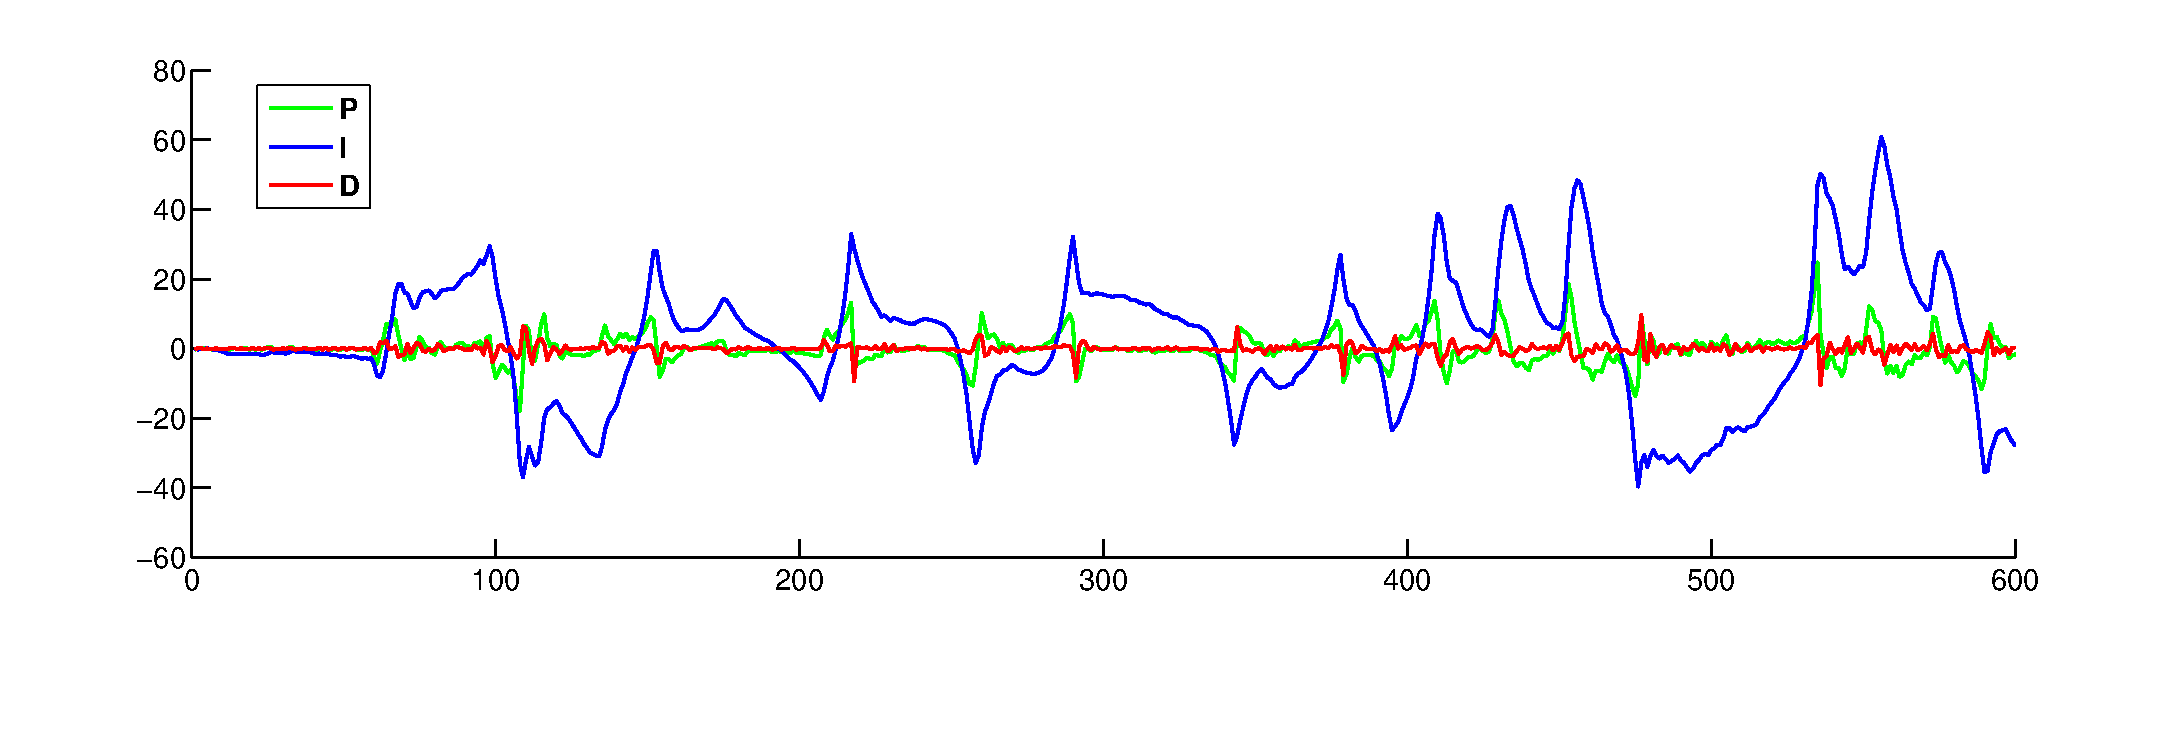
\includegraphics[width=1\linewidth]{images/pid.eps}
	\captionsetup{justification=centering,margin=1.5cm}
	\caption[Egy tesz során kapott PID tagjainak értékeit ábrázolja]
	{Egy tesz során kapott PID tagjainak értékeit ábrázolja. Az x tengelyen jelöljük a iterációk számát,	az y tengelyen a PID tagok értékének mértékét.}
	\label{pidFig}
\end{figure}

\chapter{Megvalósítás}\label{ch:MEGVALOSITAS}
\section{Elképzelések}\label{ch:MEGVALOSITAS:elkepzeles}
\section{Akadályok}\label{ch:MEGVALOSITAS:akadaly}
\section{Megoldások}\label{ch:MEGVALOSITAS:megoldas}
%\chapter{Robot programozása}\label{ch:PROG}
\section{Mindstorms}\label{sec:PROG:mindstorms}
\section{leJOS keretrendszer}\label{sec:PROG:lejos}
%\chapter{Kommunikáció és irányítás}\label{ch:KONTROLLER}
\section{Megvalósítása}\label{sec:KONTROLLER:megvalositas}
\section{Android applikáció}\label{sec:KONTROLLER:app}
\section{Protocol Buffers}\label{sec:KONTROLLER:protobuff}

%\chapter{Továbbfejleszthetőségek}
\appendix

{ 
	\renewcommand{\baselinestretch}{1.1}\normalsize %
	\setlength{\itemsep}{-2.4mm}
	\setlength{\bibspacing}{0.67\baselineskip}
	\bibliographystyle{abbrvnat_hu}
	\bibliography{dolgozat}
}


\end{document}
